\section{Selected coordinates and time-domain calculations}
\label{sec:coordinates}

\subsection{Compute pairs without building a Cartesian grid}

Use \texttt{finite\_pulse\_points} when only a diagonal cut, a few peak
coordinates, or a prescribed path through frequency space is needed. Its
signature matches \texttt{finite\_pulse\_spectrum}:
\par\noindent
\begin{minipage}{\linewidth}
\begin{lstlisting}[style=python]
finite_pulse_points(
    system, pulse1, pulse2, pulse3, omega1, omega3, T, eta,
    pathway="NR", rho0=None, signature=None,
)
\end{lstlisting}
\end{minipage}\par
Here the two frequency arrays must be one-dimensional and have equal
length. Entry $k$ requests the pair
$(\omega_1[k],\omega_3[k])$. The result has shape \texttt{(N,)} rather
than \texttt{(N, N)}. Repeated excitation and detection values are cached
internally. This API computes the full finite-pulse model; there is no
dedicated RWA selected-points wrapper in 0.2.0.

\par\noindent
\begin{minipage}{\linewidth}
\begin{lstlisting}[style=python]
cut = np.linspace(0.7, 1.5, 61)
diagonal = pulsus.finite_pulse_points(
    system=system,
    pulse1=pulse, pulse2=pulse, pulse3=pulse,
    omega1=cut, omega3=cut,
    T=20.0, eta=0.02, pathway="NR", rho0=rho_ss,
)
assert diagonal.shape == (len(cut),)
\end{lstlisting}
\end{minipage}\par
This evaluates the diagonal directly without calculating all
$61^2$ combinations. For an R diagonal in native coordinates, supply
\texttt{omega1=-cut} and \texttt{omega3=cut} with
\texttt{pathway="R"}. The pairs retain their supplied order.

When comparing points with an existing grid, preserve its row/column
ordering:
\par\noindent
\begin{minipage}{\linewidth}
\begin{lstlisting}[style=python]
rows = np.array([0, 10, 20])  # omega3 indices
cols = np.array([5, 15, 25])  # omega1 indices
values = pulsus.finite_pulse_points(
    system=system,
    pulse1=pulse, pulse2=pulse, pulse3=pulse,
    omega1=omega1[cols], omega3=omega3[rows],
    T=20.0, eta=0.02, pathway="NR", rho0=rho_ss,
)
assert np.allclose(values, S_NR[rows, cols])
\end{lstlisting}
\end{minipage}\par
The two integer arrays above select three paired entries, not a
three-by-three subgrid. The complete example is
\texttt{examples/manual/04\_selected\_points.py}.

\begin{figure}[!htbp]
\centering
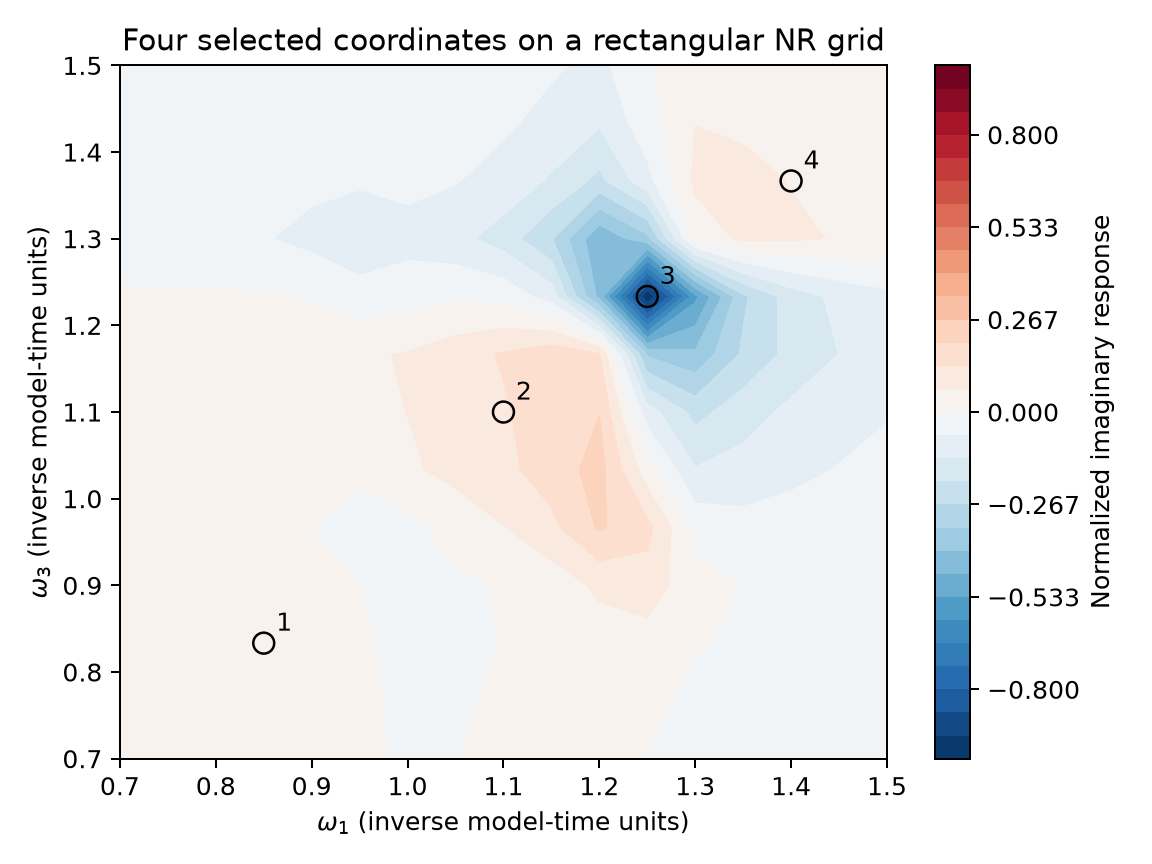
\includegraphics[width=0.75\linewidth]{figures/selected_points.png}
\caption{Four paired coordinates on a $13\times17$ Cartesian grid.
The numbered circles mark the pairs evaluated by
\texttt{finite\_pulse\_points}; their complex values agree with the
corresponding grid entries. The background is a normalized imaginary
NR response, sampled coarsely for this indexing demonstration.}
\label{fig:selected-points}
\end{figure}

\subsection{A generic grid evaluator}

\texttt{response\_grid(response\_function, omega1, omega3, **kwargs)}
calls a scalar response function for every Cartesian pair. The function
must accept \texttt{omega1} and \texttt{omega3} as keyword arguments.
For example,
\par\noindent
\begin{minipage}{\linewidth}
\begin{lstlisting}[style=python]
S_check = pulsus.response_grid(
    pulsus.impulsive_rwa_signal,
    omega1=omega1, omega3=omega3,
    system=system, T=20.0, eta=0.02,
    pathway="NR", rho0=rho_ss,
)
\end{lstlisting}
\end{minipage}\par
The return shape is again $(N_3,N_1)$. Prefer the dedicated spectrum
wrappers for routine calculations: their caching avoids rebuilding
frequency-dependent objects at every pair. The generic evaluator is useful
for an explicitly defined scalar response or a small independent check.
To obtain a few RWA coordinates, call its scalar \texttt{\_signal}
function in a loop rather than constructing a full Cartesian grid.

\subsection{Delay-domain response functions}
\label{sec:time-domain}

The public time-domain API uses impulsive interactions. It evaluates
matrix-exponential propagation, and these functions have no
\texttt{GaussianPulse} or \texttt{eta} argument. Nonnegative,
one-dimensional time axes are required. Four functions return response
arrays on delay axes:
\par\noindent
\begin{minipage}{\linewidth}
\begin{lstlisting}[style=python]
impulsive_linear_time_signal(system, times, rho0=None)
impulsive_linear_rwa_time_signal(
    system, times, sign=1, rho0=None)
impulsive_third_order_time_signal(
    system, t1, t3, T, rho0=None)
impulsive_third_order_rwa_time_signal(
    system, t1, t3, T,
    pathway="NR", signature=None, rho0=None)
\end{lstlisting}
\end{minipage}\par
The linear results have shape \texttt{(len(times),)}. The third-order
results have shape \texttt{(len(t3), len(t1))}, with nonnegative
\texttt{T}. All are complex NumPy arrays. The full-interaction third-order
response is
\begin{equation}
 R^{(3)}(t_3,T,t_1)=\langle\!\langle\mu|
 e^{\mathcal L t_3}\mathcal V e^{\mathcal L T}
 \mathcal V e^{\mathcal L t_1}\mathcal V
 |\rho_0\rangle\!\rangle.
\end{equation}
The RWA version replaces the three interactions according to the resolved
field signs and requires both dipole components.

\par\noindent
\begin{minipage}{\linewidth}
\begin{lstlisting}[style=python]
times = np.linspace(0.0, 60.0, 301)
R1 = pulsus.impulsive_linear_time_signal(
    system=system, times=times, rho0=rho_ss,
)
t1 = np.linspace(0.0, 20.0, 41)
t3 = np.linspace(0.0, 20.0, 41)
R3 = pulsus.impulsive_third_order_rwa_time_signal(
    system=system, t1=t1, t3=t3, T=20.0,
    pathway="NR", rho0=rho_ss,
)
\end{lstlisting}
\end{minipage}\par
Time axes are sampled at the values supplied; uniform spacing is not
required by the propagator API. A numerical FFT would impose additional
sampling and transform conventions that these functions do not supply.

\subsection{Laboratory-time polarization traces}

Two functions place the impulsive response on an absolute time axis:
\par\noindent
\begin{minipage}{\linewidth}
\begin{lstlisting}[style=python]
impulsive_linear_polarization(
    system, times, pulse_time=0.0, sign=None, rho0=None)
impulsive_third_order_polarization(
    system, times, pulse_times,
    pathway=None, signature=None, rho0=None)
\end{lstlisting}
\end{minipage}\par
Both return a complex vector of length \texttt{len(times)}. In the linear
function, \texttt{sign=None} uses the full interaction; $+1$ or $-1$ uses
its RWA component. The response is zero before the nonnegative
\texttt{pulse\_time} and is evaluated at delay
\texttt{times - pulse\_time} afterwards.

In the third-order function, \texttt{pulse\_times} must contain exactly
$(\tau_1,\tau_2,\tau_3)$ with
$0\leq\tau_1\leq\tau_2\leq\tau_3$. It sets
$t_1=\tau_2-\tau_1$ and $T=\tau_3-\tau_2$, and returns zero before
$\tau_3$. If both \texttt{pathway} and \texttt{signature} are
\texttt{None}, all three interactions are full. Supplying either
selects the RWA field-sign sector, with an explicit signature taking
precedence.

\par\noindent
\begin{minipage}{\linewidth}
\begin{lstlisting}[style=python]
lab_times = np.linspace(0.0, 70.0, 351)
P3 = pulsus.impulsive_third_order_polarization(
    system=system, times=lab_times,
    pulse_times=(5.0, 10.0, 30.0),
    pathway="NR", rho0=rho_ss,
)
assert np.allclose(P3[lab_times < 30.0], 0.0)
\end{lstlisting}
\end{minipage}\par
The initial state in these functions is used directly at the first
interaction. The implementation does not propagate it from laboratory
time zero to $\tau_1$ or \texttt{pulse\_time}. A stationary state is
unchanged by that omitted free interval. For a nonstationary preparation,
propagate or otherwise specify the state just before the first pulse.
These traces do not include independently specified pulse amplitudes.

\subsection{Piecewise pathway history is a different object}

The seventh public time-domain function is
\par\noindent
\begin{minipage}{\linewidth}
\begin{lstlisting}[style=python]
impulsive_pathway_polarization(
    system, times, pulse_times, pathway="NR",
    signature=None, rho0=None, return_components=False)
\end{lstlisting}
\end{minipage}\par
It always uses RWA interactions and shows successive stages of one
ordered field-sign history: first-order coherence between pulses 1 and 2,
the second-order state between pulses 2 and 3, and third-order
polarization from pulse 3 onward. The projection onto the dipole can
vanish during a stage even though the intermediate density operator is
nonzero.

With \texttt{return\_components=True}, the return value is a tuple:
\par\noindent
\begin{minipage}{\linewidth}
\begin{lstlisting}[style=python]
history, components = pulsus.impulsive_pathway_polarization(
    system=system, times=lab_times,
    pulse_times=(5.0, 10.0, 30.0),
    pathway="NR", rho0=rho_ss, return_components=True,
)
P1_stage = components["first_order"]
P2_stage = components["second_order"]
P3_stage = components["third_order"]
assert np.allclose(history, P1_stage + P2_stage + P3_stage)
\end{lstlisting}
\end{minipage}\par
The three arrays have disjoint stage masks. Earlier orders are set to
zero after their displayed stage. Thus \texttt{history} is a piecewise
diagnostic visualization, not the total physical polarization including
all simultaneously present orders and all pulse interactions. Use
\texttt{impulsive\_third\_order\_polarization} when the desired quantity
is strictly the third-order contribution after the third pulse.
The complete tutorial script
\path{examples/manual/05_time_domain.py} illustrates both objects.

\begin{figure}[!htbp]
\centering
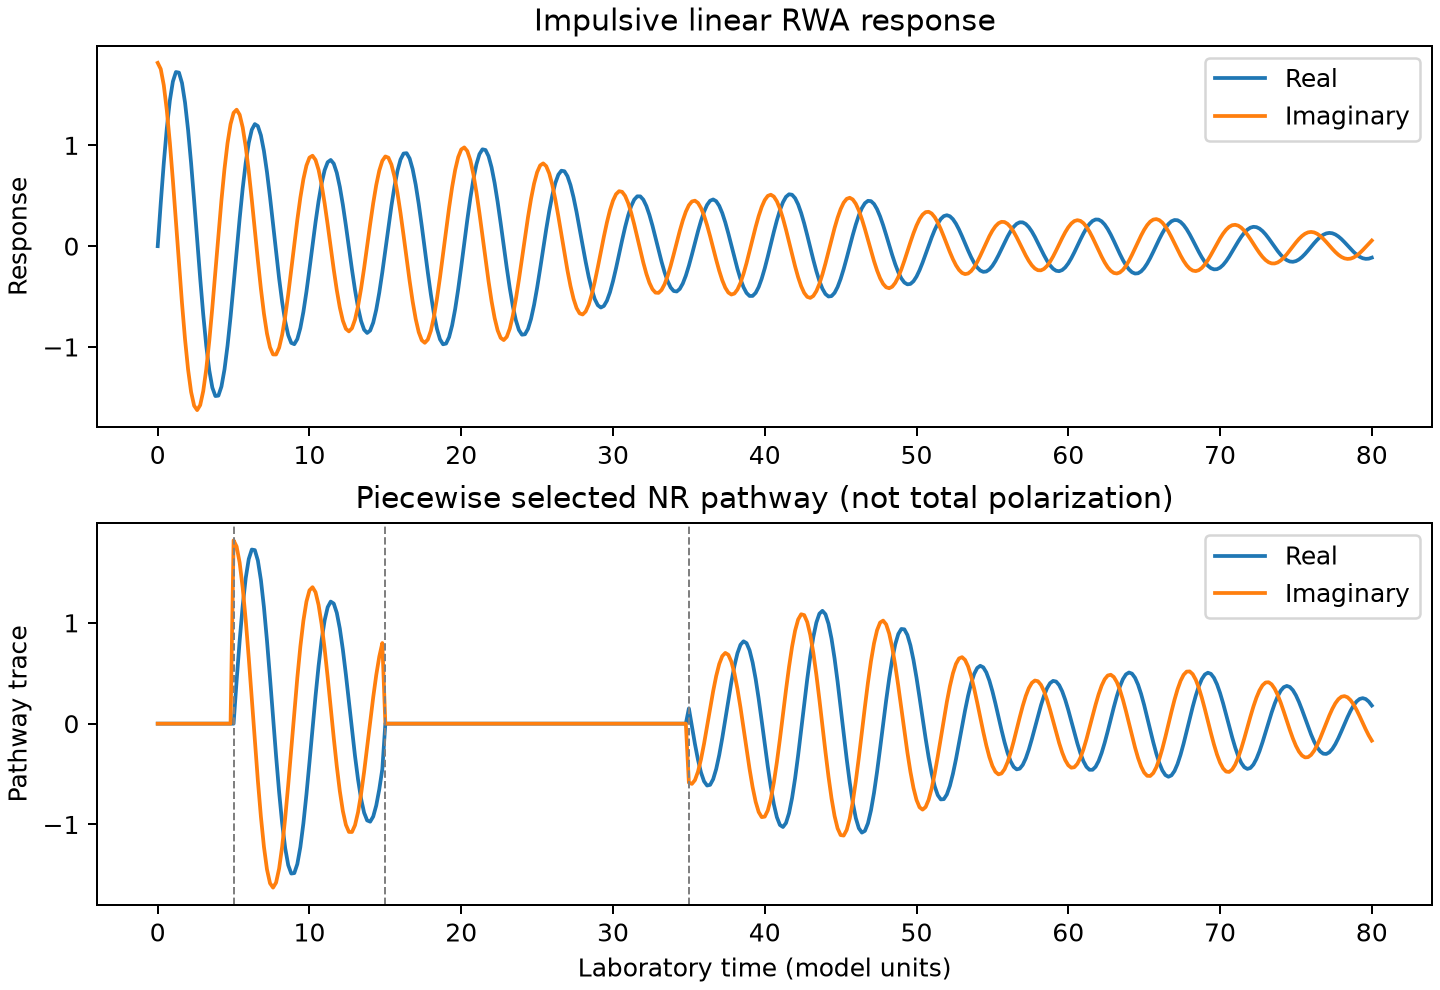
\includegraphics[width=0.9\linewidth]{figures/time_domain.png}
\caption{Impulsive linear RWA response (top) and the selected NR
pathway's piecewise history (bottom). Dashed lines mark pulses at model
times 5, 15 and 35. The stage trace after the third pulse agrees with the
strict third-order polarization for the same ordered sequence. Earlier
orders are not retained after their displayed stage.}
\label{fig:time-domain}
\end{figure}

